\documentclass[10pt,twocolumn,letterpaper]{article}

% ── Typography ────────────────────────────────────────────────────────────────
\usepackage[T1]{fontenc}
\usepackage[utf8]{inputenc}
\usepackage{newtxtext,newtxmath}      % Times-like, professional
\usepackage{microtype}                 % subtle kerning improvements
\usepackage[american]{babel}

% ── Layout ────────────────────────────────────────────────────────────────────
\usepackage[
  letterpaper,
  top=1in, bottom=1in,
  left=0.75in, right=0.75in,
  columnsep=0.30in,
]{geometry}
\usepackage{setspace}
\setlength{\parindent}{0pt}
\setlength{\parskip}{0.45em plus 0.1em minus 0.1em}

% ── Section formatting ────────────────────────────────────────────────────────
\usepackage{titlesec}
\titleformat{\section}{\large\bfseries}{\thesection}{0.6em}{}
\titleformat{\subsection}{\normalsize\bfseries}{\thesubsection}{0.6em}{}
\titlespacing*{\section}{0pt}{1.6ex plus 0.4ex minus 0.2ex}{0.8ex}
\titlespacing*{\subsection}{0pt}{1.2ex plus 0.3ex minus 0.1ex}{0.5ex}

% ── Tables ────────────────────────────────────────────────────────────────────
\usepackage{booktabs}
\usepackage{tabularx}
\usepackage{array}
\usepackage{siunitx}
\sisetup{
  group-separator={,},
  group-minimum-digits=4,
  detect-weight=true,
  detect-family=true,
}

% ── Figures and captions ──────────────────────────────────────────────────────
\usepackage{graphicx}
\usepackage[font=small,labelfont=bf,skip=4pt]{caption}
\usepackage{subcaption}
\graphicspath{{../eval/results/figures/}}

% ── Code listings ─────────────────────────────────────────────────────────────
\usepackage{listings}
\usepackage[dvipsnames]{xcolor}
\lstset{
  basicstyle=\footnotesize\ttfamily,
  frame=single,
  framesep=4pt,
  rulecolor=\color{black!40},
  numbers=none,
  breaklines=true,
  showstringspaces=false,
  xleftmargin=0pt,
  xrightmargin=0pt,
  belowskip=0pt,
  aboveskip=0pt,
}

% ── Hyperlinks (color-tweaked for print) ──────────────────────────────────────
\usepackage[colorlinks=true, allcolors=NavyBlue, breaklinks=true]{hyperref}
\usepackage{url}
\usepackage{xspace}

% ── Bibliography ──────────────────────────────────────────────────────────────
\usepackage[numbers,sort&compress,square]{natbib}
\bibliographystyle{abbrvnat}
\setlength{\bibsep}{2pt}
\renewcommand{\bibfont}{\small}

% ── Page header / footer ──────────────────────────────────────────────────────
\usepackage{fancyhdr}
\pagestyle{fancy}
\fancyhf{}
\renewcommand{\headrulewidth}{0pt}
\renewcommand{\footrulewidth}{0pt}
\fancyhead[L]{\small\itshape Preprint, May 2026}
\fancyhead[R]{\small\itshape Maurya: \distriproc}
\fancyfoot[C]{\thepage}

% ── Macros ────────────────────────────────────────────────────────────────────
\newcommand{\distriproc}{\textsc{DistriProc}\xspace}
\newcommand{\uffd}{\texttt{userfaultfd}\xspace}

% ── Title block ───────────────────────────────────────────────────────────────
\title{\vspace{-2.5em}\Large\bfseries
  \distriproc: An Adaptive Post-Restore Remote-Memory\\Runtime for Linux Processes
  \vspace{-0.4em}
}
\author{
  \large Utkarsh Maurya\\[1pt]
  \small\itshape Independent Researcher\\[1pt]
  \small\texttt{projects.utkarshmaurya@gmail.com}
  \vspace{-0.6em}
}
\date{}

% ──────────────────────────────────────────────────────────────────────────────
\begin{document}
\makeatletter
\twocolumn[
  \begin{@twocolumnfalse}
    \maketitle
    \begin{abstract}\noindent
      Checkpoint/Restore In Userspace (CRIU) supports lazy restore, which allows a
      process to resume execution before all its pages have been transferred from a
      remote page server. This reduces time-to-first-request (TTFR) dramatically for
      workloads with small active footprints at restore time, but leaves the policy
      question open: should the runtime prefetch additional pages speculatively, and
      if so, how many?

      We show that a fixed sequential prefetch policy can nearly double TTFR for
      memory-heavy workloads by congesting the TCP channel shared between fault
      resolution and speculative prefetch. We present \distriproc, an adaptive
      userspace runtime that monitors duplicate-fetch pressure and async queue depth
      within a sliding window of page faults, and disables prefetch when those signals
      indicate it is causing harm. Evaluated on three workloads---a synthetic loop,
      Redis with a 10{,}000-key dataset, and PyTorch inference---the adaptive policy
      reduces fixed-prefetch TTFR by 41\,\% (1{,}159$\!\to\!$686\,ms) on the
      memory-heavy workload while reducing prefetch volume by 20--58\,\% across all
      workloads, without regressing the others.
    \end{abstract}
    \vspace{1.2em}
  \end{@twocolumnfalse}
]
\makeatother

% ── 1. Introduction ──────────────────────────────────────────────────────────
\section{Introduction}

Cloud platforms routinely checkpoint and migrate running processes for load balancing,
preemption recovery, and live migration. CRIU~\cite{criu} provides this capability for
Linux processes without application modification. Its lazy restore mode is particularly
attractive: rather than waiting for all memory pages to be copied before resuming the
process, CRIU installs a \uffd~\cite{userfaultfd} handler that fetches pages on demand
from a remote page server. The process begins running immediately, and pages arrive as
they are accessed.

The central operational question is what fetching policy the runtime should use during
this post-restore phase. Three options exist. \emph{Pure demand paging} fetches only
what the process explicitly faults on, contributing no extra network traffic but
potentially stalling on every new page. \emph{Sequential prefetch} speculatively
fetches nearby pages after each fault, reducing future fault latency at the cost of
additional network traffic. An \emph{adaptive policy} monitors runtime signals and
switches between these behaviors based on observed conditions.

Prior deployments of CRIU lazy restore~\cite{criu-lazy,runc-lazy} have not
systematically studied the policy question. In particular, the assumption that prefetch
is always beneficial turns out to be incorrect. We demonstrate empirically that a fixed
sequential prefetch policy can nearly double TTFR for workloads with large working
sets, because speculative traffic competes with fault-path traffic over the same TCP
connection, building up an async queue backlog that delays synchronous fault
resolution.

We make three contributions:

\begin{enumerate}\itemsep2pt\parskip0pt

\item We demonstrate that lazy restore provides a 21$\times$ TTFR reduction for
memory-light workloads, but that this benefit inverts for memory-heavy workloads where
the process must page in its full working set before serving (\S\ref{sec:eval}).

\item We show that fixed sequential prefetch increases TTFR by 85\,\% for a PyTorch
inference server (625$\!\to\!$1{,}159\,ms) by reducing page faults 60\,\% while
simultaneously congesting the fault path---establishing that fault reduction is not a
reliable proxy for latency improvement (\S\ref{sec:paradox}).

\item We present an adaptive controller that uses duplicate-fetch pressure and async
queue depth as lightweight signals within a 128-fault sliding window, and show that it
recovers 473\,ms of the TTFR degradation caused by fixed prefetch on the memory-heavy
workload while cutting prefetch volume 20--58\,\% across all workloads
(\S\ref{sec:controller-eval}).

\end{enumerate}

\distriproc is implemented as a userspace daemon in approximately 1{,}200 lines of C
and 300 lines of Python. All experiments use a TCP loopback page server; RDMA, writable
remote-memory coherence, and multi-node distribution are out of scope for this paper.

% ── 2. Background ────────────────────────────────────────────────────────────
\section{Background}
\label{sec:background}

\subsection{CRIU and Lazy Restore}

CRIU checkpoints a Linux process by dumping its memory pages, file descriptors, and
kernel state to an image on disk. Restore replays this image to reconstruct the
process. \emph{Full restore} copies all memory pages into the restored process before
resuming execution. This can take hundreds of milliseconds for processes with large
address spaces.

\emph{Lazy restore} defers page transfer. At restore time, CRIU marks the process's
virtual memory regions as unpopulated and registers a \uffd file descriptor that
intercepts page faults. When the process accesses an unpopulated page, the kernel
delivers a \texttt{UFFD\_EVENT\_PAGEFAULT} event to the handler. The handler fetches
the missing page from a remote page server over TCP, installs it via
\texttt{ioctl(UFFDIO\_COPY)}, and returns control to the process. The process resumes
execution at the faulting instruction without any application-level change.

This model allows the process to begin executing within tens of milliseconds of
restore: only stack, entry-point code, and initial data must be present before the
first instruction runs. The remaining pages arrive on demand.

\subsection{Userfaultfd}

\texttt{userfaultfd(2)} is a Linux kernel mechanism (available since kernel 4.3) that
allows userspace to handle page faults for a given virtual memory range. A process
registers memory regions with a \uffd file descriptor, then reads fault events from
it. For each fault, the handler must install a page via \texttt{UFFDIO\_COPY}
(zero-copy from a userspace buffer) or \texttt{UFFDIO\_ZEROPAGE} before returning. The
faulting thread is blocked until the handler resolves the fault.

\distriproc's lazy handler polls the \uffd file descriptor on the main thread,
resolves each fault synchronously, and dispatches prefetch work to a background thread
via a bounded queue. The background thread uses a separate TCP connection to the page
server to avoid contending with synchronous fault resolution on the primary connection.

\subsection{The Post-Restore Remote-Memory Phase}

After lazy restore, the process operates in a \emph{remote-memory phase}: some pages
reside locally (those already faulted in) and the remainder reside on the page server.
This phase ends when all pages have been accessed at least once. The duration and
character of this phase depend entirely on the workload's access pattern:

\begin{itemize}\itemsep2pt\parskip0pt
\item A process that immediately touches all its memory (e.g., a model server loading
weights) will fault on virtually every page before it can serve its first request.
Lazy restore provides little TTFR benefit and exposes the full RTT of fetching each
page.

\item A process that can serve requests using a small active footprint (e.g., a loop
server that touches only its stack) will complete TTFR in milliseconds, because only a
handful of pages are needed before the first response.
\end{itemize}

This distinction motivates workload-aware policy.

% ── 3. Design ────────────────────────────────────────────────────────────────
\section{Design}
\label{sec:design}

\subsection{System Architecture}

\distriproc consists of three components.

\textbf{Page server} (\texttt{criu\_page\_server.py}): a TCP server that reads CRIU
page image files and serves individual pages on request. It accepts two connections
per restore session: one for synchronous fault resolution and one for async prefetch.

\textbf{Lazy handler} (\texttt{lazy\_handler.c}): a userspace daemon that registers
the restored process's memory regions with \uffd, then runs a main loop that reads
fault events, fetches faulted pages synchronously over TCP, and optionally queues
prefetch work for a background thread.

\textbf{Hot-page profiler} (\texttt{hot\_pages.py}): an optional pass that records the
most-accessed pages before checkpointing and passes them to the handler for eager
prefetch at restore time. Not evaluated in this paper.

\subsection{Prefetch Modes}

The handler supports three policy modes, selectable at invocation time.

\textbf{Lazy (demand-only).} No speculative fetching. Each page fault is resolved by
fetching exactly the faulted page. Minimizes network traffic but may stall on every
unique page access.

\textbf{Fixed prefetch.} After each fault on page $P$, the handler queues pages
$P{+}1, \ldots, P{+}S$ (configurable stride $S$, window $W$) to the background
prefetch thread. The prefetch thread fetches them over the secondary TCP connection if
they have not already been served. The policy is fixed: it does not observe whether
prefetch is beneficial.

\textbf{Adaptive prefetch.} Begins like fixed prefetch but activates a controller
that monitors signals within a sliding window of $N$ faults. When the controller
determines that prefetch is wasteful, it disables the prefetch thread until conditions
improve.

\subsection{Adaptive Controller}
\label{sec:controller}

The adaptive controller runs at the end of every $N$-fault window ($N=128$ in all
experiments). It observes three signals.

\textbf{Duplicate pressure} (\textit{dup\_rate}): the fraction of prefetch requests
within the current window that were for pages already served. A high duplicate rate
indicates the prefetch worker is re-requesting pages the fault path already resolved.

\textbf{Queue depth} (\textit{qdepth}): the number of unprocessed prefetch requests
waiting in the bounded queue. A large queue indicates outstanding prefetch traffic is
occupying TCP bandwidth and adding latency to the fault path.

\textbf{Queue drops}: prefetch requests dropped because the queue was full. A nonzero
count confirms the queue is saturated.

The controller logic is summarized below:

\begin{lstlisting}
if dup_rate > DUP_THRESHOLD or
   qdepth   > QDEPTH_THRESHOLD:
    disable prefetch
    wait until qdepth < DRAIN_THRESHOLD
    re-enable with small probe window
    if not wasteful: restore full W, S
    else: disable again
\end{lstlisting}

Current thresholds: \texttt{DUP\_THRESHOLD}=70\,\%, \texttt{QDEPTH\_THRESHOLD}=500,
\texttt{DRAIN\_THRESHOLD}=64. These were set by inspection of early runs and not
tuned further. The controller is intentionally simple: it is a first paper-worthy
policy, not a final production one.

\textbf{Why not hit rate?}\, An intuitive signal would be the fraction of prefetched
pages subsequently faulted on. In practice this metric is unreliable for async
prefetch: if the worker installs a page before the fault fires, no event registers the
installation as a hit. In all our experiments, the reported hit rate is 0\,\% despite
active prefetch. The controller therefore uses duplicate pressure and queue depth
instead.

% ── 4. Implementation ────────────────────────────────────────────────────────
\section{Implementation}
\label{sec:impl}

\subsection{Fault Path}

The main handler thread polls \uffd with a 1-second timeout. On each fault event, it
checks a shared hash set of already-served pages (\S\ref{sec:sharedstate}). If served,
it calls \texttt{ioctl(UFFDIO\_COPY)} from local cache. Otherwise it sends a request
over the primary TCP connection, reads the page data, and installs it via
\texttt{UFFDIO\_COPY}. The faulting thread is unblocked as soon as
\texttt{UFFDIO\_COPY} returns.

\subsection{Async Prefetch Path}

After resolving a fault on page $P$, the handler computes prefetch candidates and
attempts to push each to a bounded MPSC queue shared with the prefetch thread. If the
queue is full, the request is dropped and a drop counter is incremented.

The prefetch thread dequeues candidates in order. For each candidate, it checks the
shared hash set. If the page is already served, it increments the duplicate counter
and discards the request. Otherwise it fetches the page over the secondary TCP
connection, installs it via \texttt{UFFDIO\_COPY}, and marks it as served.

This architecture ensures the primary fault path is never blocked by prefetch
activity: the two TCP connections are independent, and the queue bounds the memory
footprint of outstanding requests.

\subsection{Shared State}
\label{sec:sharedstate}

The served-page set is a fixed-size open-addressing hash set
(\texttt{hashset.h}). Access is protected by a mutex. Both the fault path (to avoid
re-fetching pages already installed by the prefetch thread) and the prefetch thread
(to skip duplicate requests) consult it. Contention is low because the prefetch
thread operates at a slower pace than the fault path on most workloads.

\subsection{Lifecycle Events}

The \uffd protocol generates non-fault events (\texttt{UFFD\_EVENT\_UNMAP},
\texttt{REMAP}, \texttt{REMOVE}, \texttt{FORK}) in addition to page faults.
\distriproc handles these explicitly: it logs \texttt{UNMAP} events and exits cleanly
on restore completion.

% ── 5. Evaluation ────────────────────────────────────────────────────────────
\section{Evaluation}
\label{sec:eval}

\subsection{Setup}

\textbf{Hardware:} AMD Ryzen 7 7735HS (8 cores), 15\,GB RAM, x86\_64.\, \textbf{Software:} Linux 6.18.7, CRIU 4.2, Python 3, PyTorch (CPU-only).\, \textbf{Transport:} TCP loopback (127.0.0.1). All experiments run on a single machine; this represents best-case network conditions.\, \textbf{Methodology:} Each configuration runs 5 iterations. We report mean $\pm$ standard deviation. TTFR is measured from the moment \texttt{criu restore} is invoked to the moment the workload responds to a probe request.

\textbf{Workloads.}
\begin{itemize}\itemsep2pt\parskip0pt
\item \textbf{test\_loop}: a synthetic C process that increments a counter in a tight
loop and responds to a UDP probe. Footprint $\approx$266 pages ($\approx$1\,MB).

\item \textbf{Redis}: Redis 7.x pre-warmed with 10{,}000 unique keys
($\approx$13.77\,MB working set). Throughput measured as GET ops/sec via
\texttt{redis-benchmark}.

\item \textbf{PyTorch}: ResNet-18 loaded into memory, checkpointed, and lazily
restored. Footprint $\approx$15{,}743 pages ($\approx$61\,MB).
\end{itemize}

\textbf{Modes.} \texttt{full} (CRIU full restore), \texttt{lazy} (demand-only),
\texttt{lazy-prefetch} (fixed window=16, stride=8), \texttt{lazy-adaptive} (same
window/stride, adaptive controller).

\subsection{Time-to-First-Request}
\label{sec:eval-ttfr}

Table~\ref{tab:ttfr} summarizes TTFR across all workloads and modes;
Figure~\ref{fig:pytorch_ttfr} shows the PyTorch result;
Figure~\ref{fig:ttfr_all} shows all three workloads.

\begin{table}[t]
\centering
\caption{Mean TTFR (ms) $\pm$ stddev, $n=5$. H1 threshold: ${<}1000$\,ms.}
\label{tab:ttfr}
\small
\begin{tabular}{l S[table-format=4.0] @{\,$\pm$\,} S[table-format=2.0] S[table-format=4.0] @{\,$\pm$\,} S[table-format=2.0] S[table-format=4.0] @{\,$\pm$\,} S[table-format=2.0] S[table-format=4.0] @{\,$\pm$\,} S[table-format=2.0]}
\toprule
{Workload} & \multicolumn{2}{c}{Full} & \multicolumn{2}{c}{Lazy} & \multicolumn{2}{c}{Fixed} & \multicolumn{2}{c}{Adaptive} \\
\midrule
test\_loop & 1020 & 2  & 48   & 4  & 48   & 4  & 49  & 6  \\
Redis      & 32   & 1  & 46   & 10 & 38   & 9  & 44  & 6  \\
PyTorch    & 209  & 11 & 625  & 18 & 1159 & 24 & 686 & 67 \\
\bottomrule
\end{tabular}
\end{table}

\begin{figure}[t]
  \centering
  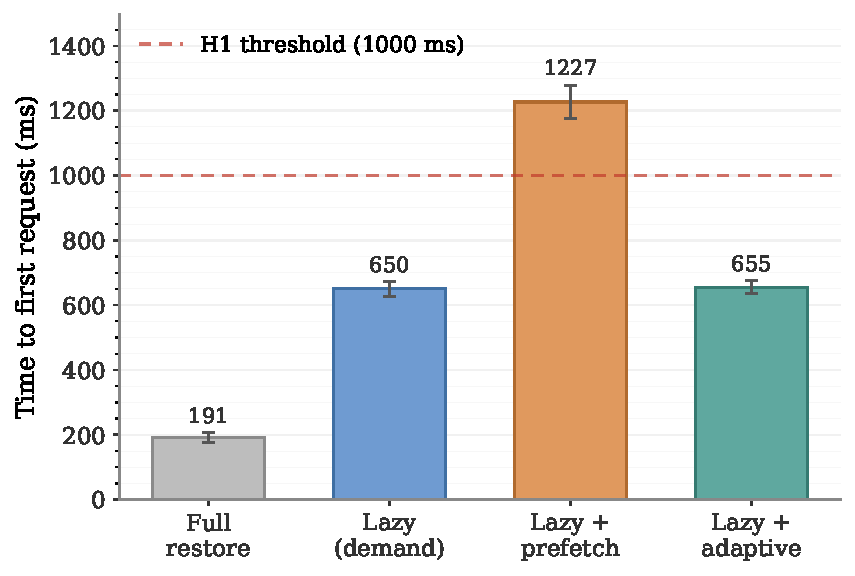
\includegraphics[width=\columnwidth]{fig1_pytorch_ttfr.pdf}
  \caption{PyTorch TTFR across restore modes. Fixed prefetch nearly doubles TTFR;
    adaptive recovers to 686\,ms. Dashed line: H1 threshold (1000\,ms).}
  \label{fig:pytorch_ttfr}
\end{figure}

\textbf{test\_loop.}\, Lazy restore is 21$\times$ faster than full (48 vs.\ 1020\,ms).
The active footprint at restore time is tiny: only stack and code pages are needed
before the first response. All three lazy modes are statistically indistinguishable
(48, 48, 49\,ms), confirming prefetch has neither benefit nor harm on a small working
set.

\textbf{Redis.}\, Lazy restore is marginally slower than full (46 vs.\ 32\,ms). Redis
can respond before most pages are faulted in. All modes pass H1 comfortably.

\textbf{PyTorch.}\, This workload exhibits the failure mode of fixed prefetch. Full
restore completes in 209\,ms. Lazy restore takes 625\,ms because ResNet-18 weights
($\approx$15{,}000 pages, $\approx$61\,MB) must all be paged in before the first
inference. Fixed prefetch worsens TTFR to 1{,}159\,ms---an 85\,\% regression over
demand-only and 5.5$\times$ over full restore---despite reducing page fault count by
60\,\% (15{,}743$\!\to\!$6{,}352). The adaptive controller brings TTFR back to
686\,ms ($-$473\,ms vs.\ fixed prefetch, $-$41\,\%), within 10\,\% of demand-only.

\begin{figure*}[t]
  \centering
  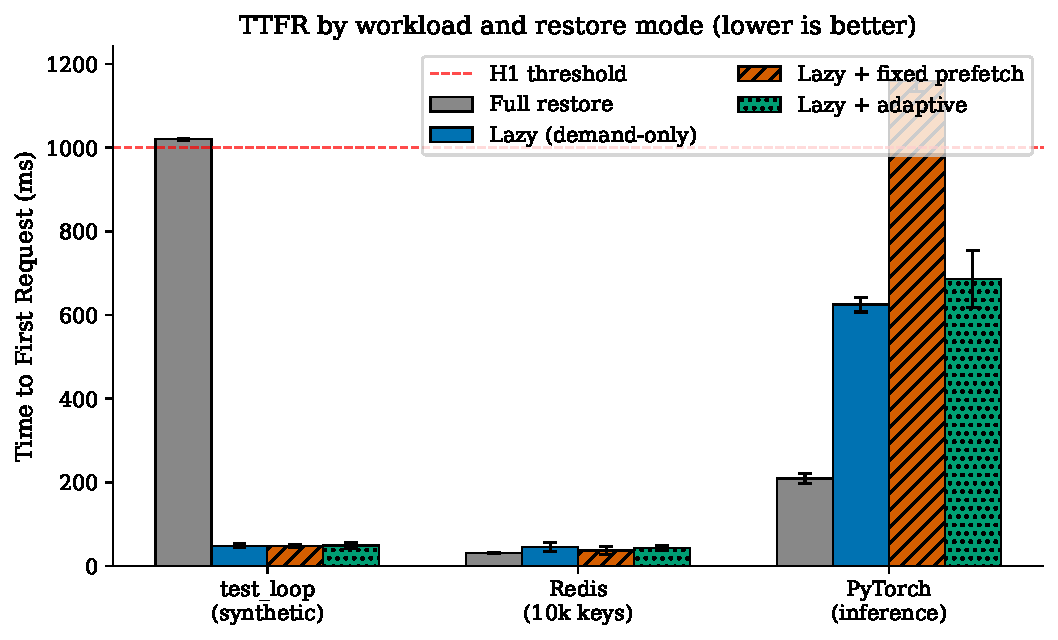
\includegraphics[width=0.78\textwidth]{fig2_ttfr_all.pdf}
  \caption{TTFR by workload and restore mode. Lazy is 21$\times$ faster than full on
    test\_loop (small footprint), marginally slower on Redis, 3$\times$ slower on
    PyTorch (must page in full working set before serving).}
  \label{fig:ttfr_all}
\end{figure*}

\subsection{The Fixed-Prefetch Paradox}
\label{sec:paradox}

Fixed prefetch on PyTorch reduces page faults by 60\,\% yet nearly doubles TTFR
(Figure~\ref{fig:faults_vs_ttfr}). This apparent paradox is explained by TCP channel
dynamics. The prefetch worker generates a backlog of pending TCP reads on the
secondary connection. Although this does not directly block the primary connection,
it congests the kernel's socket send buffer for the page server, delaying responses
on the primary connection. The effect manifests as growing \textit{qdepth} and
ultimately increases wall-clock time per fault.

The 60\,\% fault reduction is real: fewer faults fire. But the remaining 40\,\% take
longer to resolve because each resolution is delayed by congestion. The net effect is
higher TTFR.

\begin{figure*}[t]
  \centering
  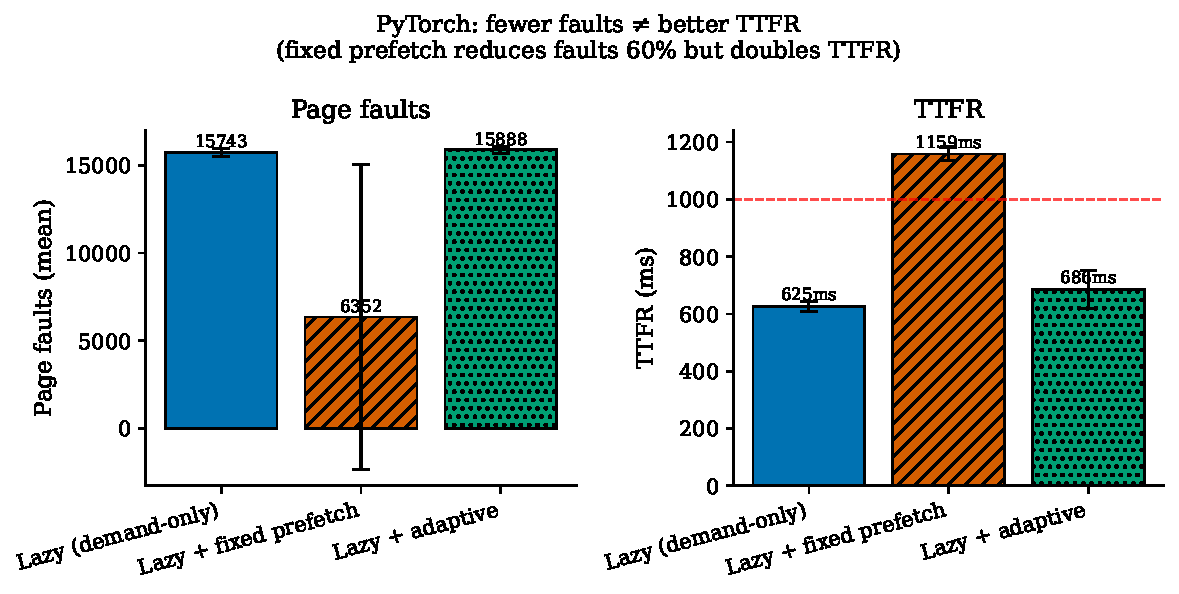
\includegraphics[width=0.78\textwidth]{fig4_faults_vs_ttfr.pdf}
  \caption{PyTorch page faults vs.\ TTFR. Fixed prefetch reduces faults 60\,\% but
    nearly doubles TTFR. Fewer faults do not imply lower latency when prefetch
    congests the fault-path TCP channel.}
  \label{fig:faults_vs_ttfr}
\end{figure*}

\subsection{Adaptive Controller Behavior}
\label{sec:controller-eval}

\textbf{PyTorch.}\, The controller observes 5 control windows (640 faults) before
disabling prefetch (Table~\ref{tab:controller}, Figure~\ref{fig:timeline}). It
progressively reduces window and stride before disabling at window 5, when duplicate
rate is 100\,\% and queue depth has grown to 3{,}796.

\begin{table}[t]
\centering
\caption{PyTorch adaptive controller windows (iteration 1).}
\label{tab:controller}
\small
\begin{tabular}{c S[table-format=3.0] S[table-format=4.0] l}
\toprule
{Window} & {Dup rate (\%)} & {Queue depth} & {Decision} \\
\midrule
1 & 100 & 2704 & on (reduce $W,S$) \\
2 & 78  & 3288 & on (reduce $W,S$) \\
3 & 100 & 3552 & on (reduce $W,S$) \\
4 & 100 & 3714 & on (reduce $W,S$) \\
5 & 100 & 3796 & \textbf{off}      \\
\bottomrule
\end{tabular}
\end{table}

The adaptive mode's fault count (15{,}888) is nearly identical to demand-only
(15{,}743), confirming the controller backed off almost completely after the probe
window.

\textbf{Redis.}\, The controller disables prefetch in a single window: 94\,\%
duplicate rate, queue depth 821. Redis's access pattern is essentially random across
10{,}000 keys; sequential prefetch predicts nothing and every prefetch candidate is
already served by the time the worker processes it.

\begin{figure*}[t]
  \centering
  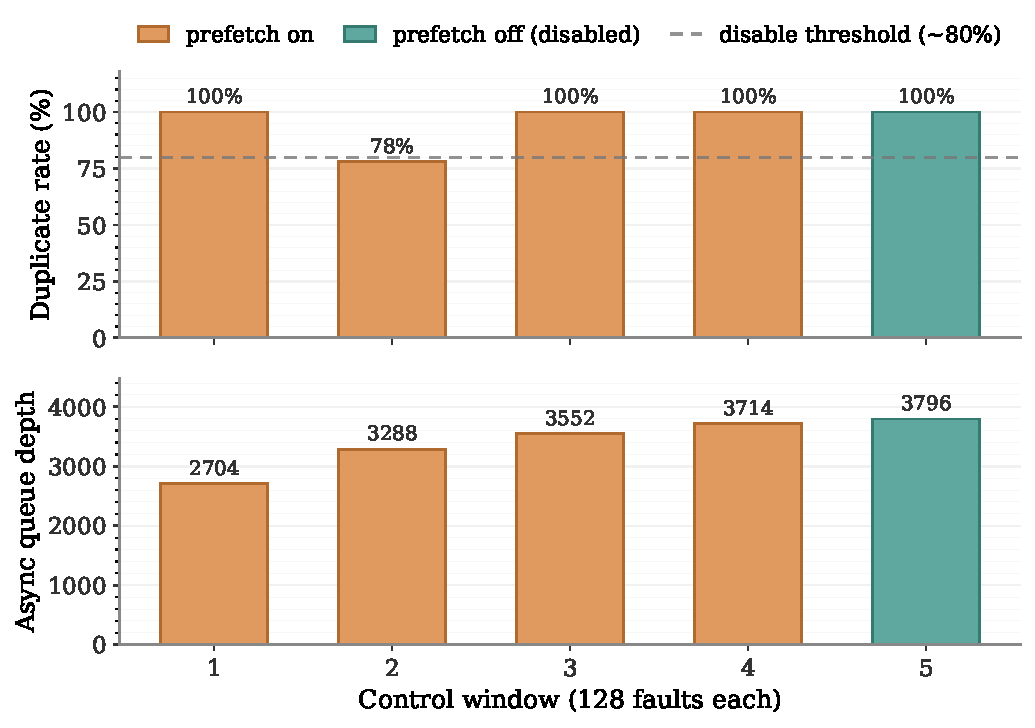
\includegraphics[width=0.78\textwidth]{fig5_adaptive_timeline.pdf}
  \caption{Adaptive controller decisions per 128-fault window (PyTorch, iteration 1).
    Duplicate rate stays at 100\,\% and queue depth climbs across windows; the
    controller progressively reduces window/stride before disabling at window 5.}
  \label{fig:timeline}
\end{figure*}

\subsection{Throughput}

\begin{table}[t]
\centering
\caption{Throughput. Percentages relative to full restore baseline.}
\label{tab:throughput}
\small
\begin{tabular}{l r r r r}
\toprule
Workload & Full & Lazy & Fixed & Adaptive \\
\midrule
test\_loop & 1\,op/s    & 100\,\% & 100\,\% & 100\,\% \\
Redis      & 107{,}146  & 68\,\%  & 66\,\%  & 69\,\%  \\
PyTorch    & 84\,inf/s  & 100\,\% & 97\,\%  & 94\,\%  \\
\bottomrule
\end{tabular}
\end{table}

All lazy modes achieve $\geq$94\,\% of full restore throughput on PyTorch and
test\_loop. Redis lazy modes reach 68--69\,\%. This shortfall reflects TCP transport
overhead: Redis issues random GET operations that touch pages across the working set,
each requiring a TCP round-trip. All lazy modes show roughly equal Redis throughput,
confirming this is a transport limitation, not a policy effect.

\textbf{PyTorch throughput caveat.}\, Throughput is measured after the post-restore
phase concludes, on the restored process. All modes converge once pages are local;
the numbers (79--84 inferences/sec) reflect CPU-bound inference speed.

\subsection{Prefetch Volume Reduction}

\begin{table}[t]
\centering
\caption{Mean prefetch volume per restore session.}
\label{tab:prefetch}
\small
\begin{tabular}{l S[table-format=5.0] S[table-format=5.0] r}
\toprule
{Workload} & {Fixed} & {Adaptive} & {Reduction} \\
\midrule
test\_loop & 76    & 32    & $-$58\,\% \\
Redis      & 1579  & 874   & $-$45\,\% \\
PyTorch    & 2121  & 1695  & $-$20\,\% \\
\bottomrule
\end{tabular}
\end{table}

The adaptive controller reduces prefetch volume on all three workloads
(Figure~\ref{fig:prefetch_vol}), even on test\_loop where fixed prefetch causes no
measurable harm. The PyTorch reduction is smaller ($-$20\,\%) because most prefetch
volume occurs in the early probe windows before the controller disables.

\begin{figure}[t]
  \centering
  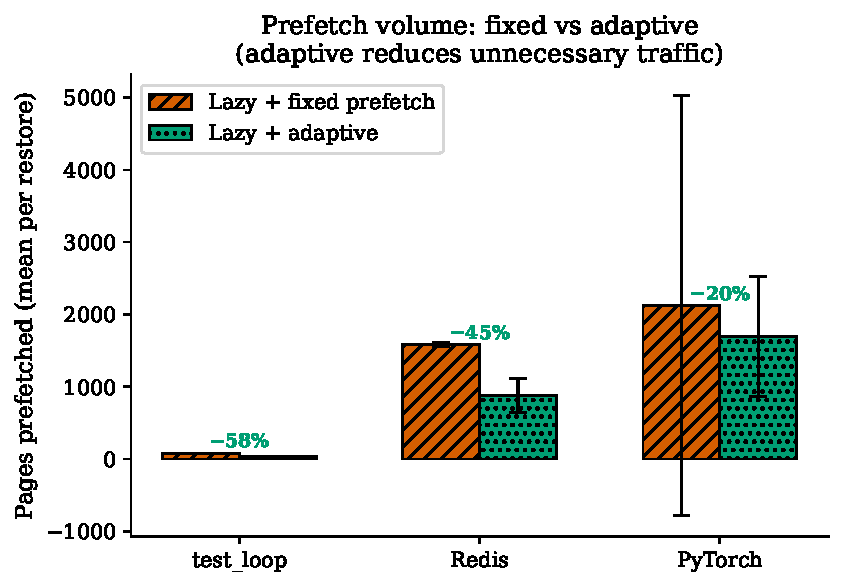
\includegraphics[width=\columnwidth]{fig3_prefetch_volume.pdf}
  \caption{Prefetch volume per restore session. Adaptive cuts volume 20--58\,\%
    across workloads with negligible TTFR penalty on test\_loop and Redis.}
  \label{fig:prefetch_vol}
\end{figure}

% ── 6. Discussion ────────────────────────────────────────────────────────────
\section{Discussion}
\label{sec:discussion}

\textbf{When lazy restore helps and when it does not.}\, Lazy restore is most
beneficial for processes that can satisfy their first requests using a small fraction
of their address space. For test\_loop, TTFR is determined by kernel restore overhead
and a handful of pages, and lazy restore eliminates the page-copy phase entirely
(21$\times$ speedup). For PyTorch inference, the process cannot serve its first
request until all $\approx$15{,}000 model weight pages are local, and lazy restore
imposes a 3$\times$ TTFR overhead relative to full restore. This workload dependence
is fundamental; we do not claim lazy restore universally reduces TTFR.

\textbf{Why adaptive recovers but does not fully match lazy.}\, On PyTorch, adaptive
mode (686\,ms) does not fully recover to demand-only lazy (625\,ms). The 61\,ms gap
comes from probe windows before the controller disables prefetch: during
$5{\times}128=640$ faults, the prefetch worker is active and building queue depth,
adding latency. A more aggressive threshold would disable prefetch sooner at the cost
of false positives. The current threshold is conservative; tuning it is left as
future work.

\textbf{Duplicate pressure as an adaptive signal.}\, Duplicate pressure is effective
because it directly measures wasted work without requiring knowledge of the
workload's access pattern. A high duplicate rate means the prefetch worker is
fetching pages the fault path has already resolved---the workload is accessing memory
in an order the sequential policy did not predict. Queue depth amplifies this signal:
even moderate duplicate pressure becomes harmful when the queue is large, because
queued-but-useless requests occupy TCP bandwidth. The combination handles both
fast-saturating workloads (Redis: single window, immediate disable) and
slow-to-saturate ones (PyTorch: 5 windows, progressive reduction).

% ── 7. Related Work ──────────────────────────────────────────────────────────
\section{Related Work}
\label{sec:related}

\textbf{CRIU and lazy restore.}\, CRIU~\cite{criu} is the standard checkpoint/restore
tool for Linux. Lazy restore via \uffd was introduced to avoid blocking restore on
large memory copies~\cite{criu-lazy}. Existing CRIU deployments do not include an
adaptive prefetch policy; the default behavior is demand-only.

\textbf{Remote memory systems.}\, Infiniswap~\cite{gu2017infiniswap} and
Fastswap~\cite{amaro2020can} implement transparent remote memory over RDMA by
replacing kernel swap with remote page fetch. AIFM~\cite{ruan2020aifm} exposes far
memory to applications via a runtime API. These systems operate at the swap or
application level and are not specific to the post-restore phase. \distriproc
operates entirely in userspace and targets the transient remote-memory state that
exists between restore and working-set convergence.

\textbf{Prefetch policies.}\, Sequential and stride prefetching in virtual memory
systems are well-studied~\cite{chen1995effective}. Adaptive prefetch has been
explored in hardware prefetchers~\cite{srinath2007feedback} and database buffer
management~\cite{cao1994influence}. To our knowledge, adaptive prefetch policy for
the \uffd post-restore phase has not been previously studied.

\textbf{Container live migration.}\, RunC and Podman support CRIU-based container
migration~\cite{runc-lazy}. Page server implementations are typically stateless TCP
servers similar to ours. No published work evaluates adaptive fetch policy for
container migration TTFR.

\textbf{Disaggregated memory.}\, LegoOS~\cite{shan2018legoos} disaggregates CPU,
memory, and storage across separate physical components. CXL-based memory
pooling~\cite{cxl} is an emerging hardware approach. \distriproc is complementary: it
provides a userspace policy layer that could sit above a CXL-backed or RDMA-backed
far-memory transport.

% ── 8. Limitations ───────────────────────────────────────────────────────────
\section{Limitations}
\label{sec:limitations}

\textbf{Transport.}\, All experiments use TCP loopback. RDMA would reduce per-page
RTT from $\approx$10\,$\mu$s to $\approx$1--2\,$\mu$s, changing absolute TTFR numbers
and likely reducing the congestion effect that makes fixed prefetch harmful. Whether
the adaptive controller remains necessary under RDMA is an open question.

\textbf{Writable coherence.}\, \distriproc does not implement write-back or
write-through to the page server. Pages installed via \texttt{UFFDIO\_COPY} are local
copies; modifications are not propagated. The system supports read-only remote memory
only.

\textbf{Controller generalization.}\, Thresholds were set by inspection on three
workloads and were not cross-validated. A workload with a mixed access pattern may
behave unpredictably. The controller is a heuristic; it is not learned.

\textbf{PyTorch throughput measurement.}\, Throughput is measured after all pages are
local. It does not capture inference throughput during the remote-memory phase.

\textbf{Single-machine evaluation.}\, Page server and process run on the same host.
True live migration across machines would expose real network RTT and bandwidth
constraints not present in loopback experiments.

% ── 9. Conclusion ────────────────────────────────────────────────────────────
\section{Conclusion}
\label{sec:conclusion}

We presented \distriproc, an adaptive post-restore remote-memory runtime built on
CRIU lazy restore and \uffd. We showed that fixed sequential prefetch can nearly
double TTFR for memory-heavy workloads by congesting the fault-path TCP channel, and
that a simple per-window controller using duplicate pressure and queue depth can
detect and disable wasteful prefetch, recovering the majority of the performance
loss. On three workloads, the adaptive policy reduces prefetch volume 20--58\,\%
relative to fixed prefetch while matching or recovering near-lazy performance on
TTFR. The system is implemented in userspace without kernel modifications and is
reproducible from a single \texttt{make bench-paper} invocation.

% ── Bibliography ─────────────────────────────────────────────────────────────
{\small\bibliography{references}}

\end{document}
